\documentclass[11pt,landscape]{article}
\usepackage{amssymb,amsmath,amsthm,amsfonts}
\usepackage{multicol,multirow}
\usepackage{calc}
\usepackage{physics}
\usepackage{ifthen}
\usepackage{graphicx}
\usepackage[landscape]{geometry}
\usepackage[colorlinks=true,citecolor=blue,linkcolor=blue]{hyperref}

\graphicspath{ {./images/} }

\let\eps\varepsilon
\renewcommand{\arraystretch}{1}

\newtheorem{definition}{Definition}[subsection]
\newtheorem{formula}[definition]{Formula}
\newtheorem{example}[definition]{Example}
\newtheorem{remark}[definition]{Remark}

\ifthenelse{\lengthtest { \paperwidth = 11in}}
    { \geometry{top=2em,left=2em,right=2em,bottom=2em} }
	{\ifthenelse{ \lengthtest{ \paperwidth = 297mm}}
		{\geometry{top=1cm,left=1cm,right=1cm,bottom=1cm} }
		{\geometry{top=1cm,left=1cm,right=1cm,bottom=1cm} }
	}
\pagestyle{empty}
\makeatletter
\renewcommand{\section}{\@startsection{section}{1}{0mm}%
                                {-1ex plus -.5ex minus -.2ex}%
                                {0.5ex plus .2ex}%x
                                {\normalfont\large\bfseries}}
\renewcommand{\subsection}{\@startsection{subsection}{2}{0mm}%
                                {-1explus -.5ex minus -.2ex}%
                                {0.5ex plus .2ex}%
                                {\normalfont\normalsize\bfseries}}
\renewcommand{\subsubsection}{\@startsection{subsubsection}{3}{0mm}%
                                {-1ex plus -.5ex minus -.2ex}%
                                {1ex plus .2ex}%
                                {\normalfont\small\bfseries}}
\makeatother
\setcounter{secnumdepth}{0}
\setlength{\parindent}{0pt}
\setlength{\parskip}{0pt plus 0.5ex}
% -----------------------------------------------------------------------
\begin{document}

\raggedright
\footnotesize

\begin{multicols}{3}
\setlength{\premulticols}{1pt}
\setlength{\postmulticols}{1pt}
\setlength{\multicolsep}{1pt}
\setlength{\columnsep}{2pt}

\section{Maxwell's Equations}

General definitions:

$
    c=\sqrt{\mu_0\eps_0}^{-1}=3\cdot10^8[m/s],
    \,
    \lambda=c/f\cdot\frac{1}{\sqrt{\mu_r\eps_r}},
    \,
    k=2\pi/\lambda
$

\vspace{1em}
$
    fF=10^{-15}F, \mu_0=4\pi10^{-7}[H/m], \eps_0=8.85\cdot10^{-12}[F/m]
$
\vspace{1em}

$\eta_0=\sqrt{\frac{\mu_0}{\eps_0}}=120\pi[\Omega]$

\vspace{1em}
$
    \curl A =
    \left(\pdv{A_z}{y}-\pdv{A_y}{z}\right)\vu{x}+
    \left(\pdv{A_x}{z}-\pdv{A_z}{x}\right)\vu{y}+
    \left(\pdv{A_y}{x}-\pdv{A_x}{y}\right)\vu{z}
$

\begin{align*}
    \mqty[\vu{x}\\\vu{y}\\\vu{z}]
    =
    \mqty[
        \sin\theta\cos\varphi & \cos\theta\cos\varphi & -\sin\varphi\\
        \sin\theta\sin\varphi & \cos\theta\sin\varphi & \cos\varphi\\
        \cos\theta & -\sin\theta & 0
        ]
    \mqty[\vu{r}\\\vu{\theta}\\\vu{\varphi}]
\end{align*}

\begin{align*}
    \curl A
    &=\frac{1}{r\sin\theta} \left(\pdv{A_\varphi\sin\theta}{\theta}-\pdv{A_\theta}{\varphi}\right)\vu{r}\\
    &+\frac{1}{r}\left(\frac{1}{\sin\theta}\pdv{A_r}{\varphi}-\pdv{rA_\varphi}{r}\right)\vu{\theta}\\
    &+\frac{1}{r}\left(\pdv{rA_\theta}{r}-\pdv{A_r}{\theta}\right)\vu{\varphi}
\end{align*}

trig equations:

$
\int\cos[n](\theta)\sin\theta\,d\theta=-\frac{\cos[n+1](\theta)}{n+1}
\quad
\int\sin[n](\theta)\cos\theta\,d\theta=\frac{\sin[n+1](\theta)}{n+1}
$

$
\int\sin[2](\theta)\,d\theta=\frac{2\theta-\sin(2\theta)}{4}
\quad
\int\cos[2](\theta)\,d\theta=\frac{2\theta+\sin(2\theta)}{4}
$

$
\int\sin[3](\theta)\,d\theta=\frac{\cos[3](\theta)}{3}-\cos(\theta)
\quad
\int\cos[3](\theta)\,d\theta=\sin(\theta)-\frac{\sin[3](\theta)}{3}
$

\subsection{Green's Function}

If we simplify Maxwell's in the Fourier domains, we get: $$(\nabla^2+k^2)\vec{E}=\left(j\omega\mu-\dfrac{\nabla\cdot\nabla}{j\omega\eps}\right)\vec{J}$$ To solve this, we prefer solving the Helmholtz equation $(\nabla^2+k^2)\vec{A}=-\mu\vec{J}$ and then reconstruct $\vec{E}$ and $\vec{H}$.

\begin{formula}
    A spherically symmetry Green's function for the Helmholtz equation is: $G(\vec{r}, \vec{r}\,') = g\big(\|\vec{r}-\vec{r}\,'\|\big) \approx g(r)\,\exp(jk\hat{r}\cdot\vec{r}')$
    $$g(r)=\dfrac{e^{-jkr}}{4\pi r}\Rightarrow \big[\nabla^2+ k^2\big] g(r) = -\delta(r)$$
\end{formula}

\begin{formula}
    We get the following formulas for the entire space:
    \begin{align*}
        \vec{A}(\vec{r})&=\mu\,g(\vec{r})\,\iiint\limits_V\, \vec{J}(\vec{r}\,')\,\exp( jk\hat{r}\cdot\vec{r}\,')\dd{V'}=\mu\, g(r)\,\tilde{J}(k)\\
        \vec{E}&=-j\omega\left(1+\dfrac{\nabla\cdot\nabla}{k^2}\right)\vec{A}=\dfrac{1}{j\omega\eps}\nabla\times\vec{H}\\
        \vec{H}&=\dfrac{1}{\mu}\nabla\times\vec{A}
    \end{align*}
\end{formula}

\subsection{Far Field}

\begin{formula}
    The Fraunhofer distance is $d_F=\dfrac{2D^2}{\lambda}$ where $D$ is the diameter of the antenna and $\lambda$ is the wavelength of the radio wave. If $r\gg d_F$, then we can use the far field approximation and take only the lower decaying $r$ term.
\end{formula}

\begin{formula}
    General far field structure is: $\vec{H}(r)=\frac{g(r)}{\eta}\{\hat{\varphi}E_\theta(\theta, \varphi)-\hat{\theta}E_\varphi(\theta, \varphi)\}$ and $\vec{E}=g(r)\{\hat{\theta}E_\theta(\theta, \varphi)+\hat{\varphi}E_\varphi(\theta, \varphi)\}$. Moreover, $\vec{E}=-j\omega\vec{A}_T$ (where $T$ stands for transverse component).
\end{formula}

\subsection{Polarization}

\begin{formula}
    Linear polarization: A plane wave of the form $\vec{E}=(E_x\hat{x}+E_2\hat{y})\,e^{-jkz}$ is linearly polarized at an angle of $\varphi=\arctan(E_2/E_1)$.
\end{formula}

\begin{formula}
    Circular polarization: $\vec{E}=E_0(\hat{x}\mp j\hat{y})\,e^{-jkz}$ is circularly polarized and it is right-handed on $(-)$ and left-handed on $(+)$.
\end{formula}

\begin{formula}
    Elliptical polarization: $\vec{E}=(E_{x0}\,\hat{x}+ E_{y0}\,e^{j\Delta\varphi}\,\hat{y})\,e^{-jkz}$ has axis tilt (off the $y$ axis) $\tau=\dfrac{\pi}{2}-\dfrac{1}{2}\arctan\left[\dfrac{2E_{x0}E_{y0}}{E_{x0}^2-E_{y0}^2}\cos(\Delta\varphi)\right]$ and axial ratio $AR=\dfrac{OA_+}{OA_-}$ (ratio of major to minor axis), where $OA_{\pm} = \sqrt{\frac{1}{2}\left[E_{x0}^2+E_{y0}^2\pm\sqrt{E_{x0}^4+E_{y0}^4+2E_{x0}^2E_{y0}^2\cos(2\Delta\varphi)}\,\right]}$.
\end{formula}

\begin{formula}
    The Polarization loss factor (PLF) is $\text{PLF}=|\widehat{E}_{inc}\cdot\widehat{E}_a|^2=|\widehat{\rho}_{inc}\cdot\widehat{\rho}_a|^2$ where $\vec{E}_{inc}$ is the incident wave and $\vec{E}_a$ is the transmitting wave.
\end{formula}


$\widehat{\rho_a}=\frac{\tilde{\rho_a}}{|\tilde{\rho_a}|}\, ,\va*{E_a}=\va*{\rho_a}=(x_a\vu{x}+jy_a\vu{y})f(r,\theta,\varphi)=\tilde{\rho_a}f(r,\theta,\varphi)$

\subsection{Radiation Parameters}

\begin{formula}
    We define the following parameters for an antenna:
    \begin{itemize}
        \item Poynting Vector: $\vec{S}=\dfrac{1}{2}\vec{E}\times\vec{H}^*=\dfrac{\|\vec{E}\|^2}{2\eta}\hat{r}$.
        \item Radiation Pattern: $F(\theta, \varphi) = \dfrac{\|\vec{E}(\theta,\varphi)\|}{\|\vec{E}_\text{max}\|}$.
        \item Radiation Intensity: $\displaystyle U(\theta,\varphi) = |F(\theta,\varphi)|^2=\pdv{P}{\Omega}=r^2S_r$.
        \item Power Radiated: $P_\text{rad}=\|\vec{S}\|\cdot 4\pi r^2 = \displaystyle\iint_{\Omega=0}^{4\pi}U(\theta,\varphi)\dd{\Omega}=\int\limits_{\varphi=0}^{2\pi}\int\limits_{\theta=0}^{\pi}U(\theta,\varphi)\sin\theta \,d \theta\,d\varphi$, recall $d\Omega=\sin{\theta}\dd{\theta}\dd{\varphi}$.
        \item Directivity: $D=\dfrac{U_\text{max}}{U_\text{avg}}=\dfrac{U_\text{max}}{P_\text{rad}/4\pi}$.
        \item Gain: $G=\eta D$, where $\eta$ is the efficiency of the antenna.
    \end{itemize}
\end{formula}

\begin{formula}
    Looking at the radiation pattern, we indicate the following values:
    \begin{itemize}
        \item Main lobe: $\max|F(\theta,\varphi)|$.
        \item Side Lobe Level (SLL): $20\log_{10}\left(\dfrac{F_\text{sidelobe}}{F_\text{max}}\right)$
    \end{itemize}
\end{formula}

\subsection{Hertzian dipole}

This antenna is defined by current density $\vec{J}=I_0\ell \delta(x)\delta(y)\hat{z}\Rightarrow \tilde{J}(k)=I_0\ell\hat{z}$.

\begin{example}
    The fields in the entire space: $\vec{A}=\mu I_0\ell g(r)\,\hat{z}\Rightarrow\vec{H}=-I_0\ell g'(r)\sin{\theta}\,\hat{\varphi}\Rightarrow \vec{E}=-\dfrac{I_0\ell}{j\omega\eps r}\left(2g'(r)\cos{\theta}\,\hat{r}-(g'(r)+r\cdot g''(r))\sin{\theta}\,\hat{\theta}\right)$.
\end{example}

\begin{example}
    The far field generated is: $\vec{H}=I_0\ell \,\dfrac{jk\,e^{-jkr}}{4\pi r}\sin{\theta}\,\hat{\varphi}=jk\,I_0\ell\, g(r)\sin\theta\,\hat{\varphi}$ and $\vec{E}=-\dfrac{I_0\ell}{j\omega\eps}\,\dfrac{k^2\,e^{-jkr}}{4\pi r}\sin{\theta}\,\hat{\theta}=\eta jk\,I_0\ell\, g(r)\sin\theta\,\hat{\theta}=\eta H_\varphi\,\hat{\theta}=-\eta\hat{r}\times\vec{H}$.
\end{example}

\begin{example}
    We calculate the following parameters for an antenna:
    \begin{itemize}
        \item Poynting Vector: $\vec{S}= (kI_0\ell)^2\left(\dfrac{\sin\theta}{4\pi r}\right)^2\dfrac{\eta}{2}$.
        \item Radiation Pattern: $F(\theta, \varphi) = \sin\theta$.
        \item Radiation Intensity: $\displaystyle U(\theta,\varphi) = \sin^2{\theta}$.
        \item Power Radiated: $P_\text{rad}=8\pi/3$.
        \item Directivity: $D=3/2$.
        \item Gain: $G=\eta D$.
    \end{itemize}
\end{example}

\noindent
For an arbitrary current in the antenna, we can still define the effective length $\vec{h}$ such that $\vec{E}=\eta\, jk\, I_0\vec{h}(\theta,\varphi)\, g(r)\hat{\theta}$, or equivalentely, $\vec{h}(\theta,\varphi)=\sin(\theta)\dfrac{\tilde{J}}{I_{in}}$ and all further formulas are still approximately valid.

\begin{formula}
    To find half-power beamwidth: $\Theta_h=2|\theta_m-\theta_h|$, where $\theta_m$ is the angle of the first maximum, and $\theta_h=\arccos[\frac{\lambda}{2\pi d}\left(-\beta\pm\frac{2.782}{N}\right)]$, and $\beta$ is the angle we are shifting our mainbeam by.
\end{formula}

\begin{example}
    $\ell=\lambda/2$ and $I(z)=I_0\cos(kz)$ in $[-\ell/2,\ell/2]$. Then, we calculate the current density: $\tilde{J}=\displaystyle\int_{-\ell/2}^{\ell/2}I_0\cos(kz')\exp(jkz'\cos(\theta))\dd{z'}=I_0\dfrac{2\cos\big(\pi/2 \cdot \cos(\theta)\big)}{k\sin^2(\theta)}$
\end{example}

\begin{example}
    Input impedance by shifting: original current: $I_e(z')=\vu{z}I_0\sin[k(l/2-|z'|)], \quad |z'|<l/2$. Then at infinitesimal distance: $I_{in}=I_0\sin[kl/2]=I_0\sin[\frac{2\pi}{\lambda}\frac{\lambda}{2}\frac{1}{2}]=I_0$, at some distance $d$ we get: $I_{in}'=I_0\sin[k(l/2-|z'|)]_{z'=l/2-d'}$. Then $z'/z=\left(I_{in}/I_{in}'\right)^2$
\end{example}

\subsection{Linear Arrays}

For $N$ Hertzian dipoles displaced by $\vec{d}$ and an electrical phase shift of $\Delta \phi$. Again, for a single dipole at $\vec{r}\,'$ in the $\hat{z}$ direction, the electric far field is: $\vec{E}=\dfrac{jk\eta I_0\ell\sin{\theta}}{4\pi r}\,e^{-jkr} \,\exp(-jk\hat{r}\cdot\vec{r}\,') \,\hat{\theta}$. Then, by linearity, 
\begin{align*}
    E_\theta&=\dfrac{jk\eta I_0\ell\sin{\theta}}{4\pi r}\,e^{-jkr}\sum_{n=0}^{N-1} e^{\,jn(k\hat{r}\cdot\vec{d}+\Delta\varphi)}\\
    &=E_0\,N\cdot \text{AF}(\psi=k\hat{r}\cdot\vec{d}+\Delta\varphi)\\
    \text{AF}(\psi)&=\dfrac{1}{N}\sum_{n=0}^{N-1}e^{\,jn\psi}=e^{\,j\frac{(N-1)}{2}\psi}\dfrac{\sin(N\psi/2)}{N\sin(\psi/2)}
\end{align*}
\noindent
Note the extra phase in the array factor (AF) is due to where the center of the array is. If the array is centered at the origin, there should be no phase. The maximums are the $\psi\in 2\pi\mathbb{Z}$.

\begin{formula}
    Progressive phase shift $\beta$ for shifting main-beam: $\beta=-kd\cos(\theta_0)$
\end{formula}

\begin{formula}
    Maximum distance between elements in linear scanning to suppress grating lobes: $d_{max}=\frac{\lambda}{1+|\cos(\theta_0)|}$
\end{formula}

\section{Radar and Transmission}

\subsection{Radiation - Friis' Equation}

\begin{formula}
    For a transmitting antenna, the effective area is $A_{eff}=\dfrac{\lambda^2}{4\pi} G_t$
\end{formula}

\begin{formula}
    For a Tx with $P_t$ power and $G_t$ gain and the Rx with $P_r$ power and $G_r$ gain.
    $$P_r=P_t\cdot\dfrac{G_t\cdot G_r}{(4\pi R/\lambda)^2}$$
\end{formula}

\begin{remark}
    $G[dBi]=10\log_{10}(G/G_{isotropic})$ (note on an isotropic antenna, $G_{isotropic}=1$), $P[dBm]=10\log_{10}(P/1[mW])$.
\end{remark}

\begin{formula}
    For a radar: $$P_r=P_t\cdot \dfrac{G_t\cdot G_r}{(4\pi R_t/\lambda)^2}\cdot\dfrac{\sigma}{4\pi R_r^2}$$ where $R_t$ and $R_r$ at the Tx and Rx distances and $\sigma$ is the cross-sectional area of the radar.
\end{formula}

\subsection{Noise Figure - Friis' Equation}

\begin{formula}
    The thermal noise at bandwidth $B$ and temperature $T$ has power $N=kTB$.
\end{formula}

\begin{formula}
    The SNR ratio of a component: $F=\dfrac{S_i/N_i}{S_o/N_o}\geq 1\Rightarrow 1+\dfrac{T_e}{T_0}=F$, where $F$ is the noise factor (or noise figure if in dB: $NF[dB]=10\log_{10}(F)$) and $T_e$ is the equivalent noise temperature.
    For an attenuator with temperature $T$, we have $T_e=(L-1)T$. We usually take $T_0=290[K]$.
\end{formula}

\begin{formula}
    The noise of a cascaded system is:
    \begin{align*}
        F=F_1+\dfrac{F_2-1}{G_1}+\dfrac{F_3-1}{G_1 G_2}+\cdots +\dfrac{F_n-1}{G_1\cdots G_{n-1}}
        \\
        \Leftrightarrow T_e=\sum_{i=1}^n\dfrac{T_i}{\prod_{j=0}^{i-1}G_j}
    \end{align*}
\end{formula}

\begin{example}
    For a component with gain $G$ and additive noise $N_a$, $F=1+\dfrac{N_a}{N_iG}$.
\end{example}

\begin{example}
    The noise temperature of an antenna $T_A=\eta T_{sky}+(1-\eta)T_{ant}$ and the receiver temperature $T_{rec}$ is calculated by Friis from cascading. Then $N_{out}=kBG_{sys}T_{sys}$ and $F_{sys}=1+\dfrac{T_{sys}}{T_0}$, where $T_{sys}=T_A+T_{rec}$.
\end{example}


\section{Waveguides}

\subsection{General Waveguide}

\begin{align*}
    VSWR=\frac{1+|\Gamma|}{1-|\Gamma|}
    \Longleftrightarrow
    |\Gamma|=\left|\frac{1-VSWR}{1+VSWR}\right|
\end{align*}

\begin{align*}
    \Gamma_L=\frac{Z_L-Z_c}{Z_L+Z_c}, &\quad 1 = \Gamma^2+T^2
    \\
    RL[dB] = -20\log_{10}(|\Gamma|)&\leftrightarrow |\Gamma|=10^{-RL/20}
    \\
    IL[dB]=-20\log_{10}(|T|)
\end{align*}

\begin{formula}
    Coax cable: $Z=\frac{1}{2\pi}\sqrt{\frac{\mu}{\eps}}\ln{\frac{b}{a}}$
\end{formula}

\begin{align*}
    \beta_{nm}&=\sqrt{k^2-k^2_{c,nm}},  k=\omega\sqrt{\mu\eps}=\frac{\omega}{c}\sqrt{\mu_r\eps_r},\\
    k_{c,nm}&=\sqrt{\left(\dfrac{n\pi}{a}\right)^2+\left(\dfrac{m\pi}{b}\right)^2},\\
    \text{cut-off}&: f_{c,nm}=\dfrac{1}{2\sqrt{\mu\eps}}\sqrt{\left(\dfrac{n}{a}\right)^2+\left(\dfrac{m}{b}\right)^2},\\
    \text{phase velocity} &: v_p=\dfrac{\omega}{\beta_{nm}}=\dfrac{1/\sqrt{\mu\eps}}{\sqrt{1-\big(f_{c,nm}/f\big)^2}},\\
    \text{group velocity} &: v_g=\dfrac{\beta_{nm}}{k}\dfrac{1}{\sqrt{\mu\eps}}\le\dfrac{1}{\sqrt{\mu\eps}}.\\
    Z_{nm}^{TE}&=\dfrac{\eta}{\sqrt{1-\big(f_{c,nm}/f\big)^2}}=\frac{k\eta}{\beta_{nm}}\\
    Z_{nm}^{TM}&=\eta\,\sqrt{1-\big(f_{c,nm}/f\big)^2}=\frac{\beta_{nm}\eta}{k}.
\end{align*}

\subsection{Dielectric slab and Microstrip}

Microstrip:
for $w/h<1$:

\begin{align*}
    \eps_{eff}&=\frac{\eps_r+1}{2}+\frac{\eps_r-1}{2}\left[\frac{1}{\sqrt{1+12h/w}}+0.04\left(1-\frac{w}{h}\right)^2\right]\\
    Z_c&=\frac{60}{\sqrt{\eps_{eff}}}\ln\left[\frac{8h}{w}+\frac{w}{4h}\right]
\end{align*}

for $w/h>1$:

\begin{align*}
    \eps_{eff}&=\frac{\eps_r+1}{2}+\frac{\eps_r-1}{2\sqrt{1+12h/w}}\\
    Z_c&=
    \frac{120\pi}
    {
        \sqrt{\eps_{eff}}
        \left[
            \frac{w}{h}+1.393+\frac{2}{3}\ln\left(\frac{w}{h}+1.444\right)
        \right]
    }
\end{align*}


\section{Circuits and Networks}

\subsection{Z and S-parameters}

\begin{formula}
    \begin{align*}
        \begin{bmatrix}V_1 \\ V_2 \end{bmatrix}=\begin{bmatrix}
            Z_{11} & Z_{12} \\ Z_{21} & Z_{22}
        \end{bmatrix}\begin{bmatrix}I_1 \\ I_2 \end{bmatrix}
        \quad & \quad
        \begin{bmatrix}V_1 \\ I_1 \end{bmatrix}=\begin{bmatrix}
            A & B \\ C & D
        \end{bmatrix}\begin{bmatrix}V_2 \\ -I_2 \end{bmatrix} \\
        \\
        \begin{bmatrix}b_1 \\ b_2 \end{bmatrix}=\begin{bmatrix}
            S_{11} & S_{12} \\ S_{21} & S_{22}
        \end{bmatrix}\begin{bmatrix}a_1 \\ a_2 \end{bmatrix}
        \quad & \quad
        \begin{bmatrix}b_1 \\ a_1 \end{bmatrix}=\begin{bmatrix}
            T_{11} & T_{12} \\ T_{21} & T_{22}
        \end{bmatrix}\begin{bmatrix}a_2 \\ b_2 \end{bmatrix}
    \end{align*}
    Where $a_1=V_1^+$ and $b_1=V_1^-$.
\end{formula}

\begin{formula}
    Note that $T$ and $ABCD$ cascade by matrix multiplication.
    \begin{align*}
        [ABCD]&=\dfrac{1}{Z_{21}}\begin{bmatrix}
            Z_{11} & Z_{22}\cdot Z_{11} - Z_{12}\cdot Z_{21}\\
            1 & Z_{22}
        \end{bmatrix} \\ &\Leftrightarrow
        [Z]=\dfrac{1}{C}\begin{bmatrix}
            A & AD-BC\\
            1 & D
        \end{bmatrix}\\
        [T]&=\dfrac{1}{S_{21}}\begin{bmatrix}
            S_{12}\cdot S_{21} - S_{11}\cdot S_{22} & S_{11}\\
            -S_{22} & 1
        \end{bmatrix} \\ &\Leftrightarrow
        [S]=\dfrac{1}{T_{22}}\begin{bmatrix}
            T_{12} & T_{11}\cdot T_{22} - T_{12}\cdot T_{21}\\
            1 & -T_{21}
        \end{bmatrix}
    \end{align*}
\end{formula}

\begin{example}
    For a shunt admittance, $[ABCD]=\begin{bmatrix}1 & 0 \\ Y & 1\end{bmatrix}$ and for a series impedance, $[ABCD]=\begin{bmatrix}1 & Z \\ 0 & 1\end{bmatrix}$. In a transmission line with $\gamma=\alpha+j\beta$, $[ABCD]=\begin{bmatrix}\cosh(\gamma\ell) & Z_0\sinh(\gamma\ell) \\ Y_0\sinh(\gamma\ell) & \cosh(\gamma\ell)\end{bmatrix}$.
\end{example}

\begin{example}
    $\begin{bmatrix}a_2 \\ b_2\end{bmatrix}=\begin{bmatrix}\rho_L \\ 1\end{bmatrix}V\Rightarrow \dfrac{b_1}{a_1}=\dfrac{(S_{12}\cdot S_{21} - S_{11}\cdot S_{22})\cdot \rho_L + S_{11}}{S_{21}\cdot(-S_{22}\rho_L+1)}=S_{11}+\dfrac{S_{12}S_{21}\rho_L}{1-S_{22}\rho_L}$.
\end{example}

\begin{formula}
    A network is reciprocal if $[S]^t=[S]$ and a network is lossless if $[S]^*[S]=[I]$.
\end{formula}

\begin{formula}
    The reflection coefficient is $\Gamma=S_{11}$ and the transmission is $T=S_{21}$, note $1=|\Gamma|^2+|T|^2$ if the network is lossless. Insertion loss is $\text{IL}=-20\log_{10}|S_{21}|[dB]$ and Return loss is $\text{RL}=-20\log_{10}|S_{11}|[dB]$.
\end{formula}

\subsection{Amplifiers and Mixers}

\begin{formula}
    For a mixer (depicted with $\otimes$) with oscillator frequency $f_{LO}$ and input signal $V_{in}=\sum\limits_{n\geq 0}V_n\cos(2\pi nf t)\Rightarrow$ $V_{out}=V_{in}\cdot \cos(2\pi f_{LO} t)$ $=\sum\limits_{n\geq 0}V_n\dfrac{\cos(2\pi (nf - f_{LO}) t)+\cos(2\pi (nf+f_{LO})t)}{2}$
    If we ignore the higher frequencies, we get $f-f_{LO}$.
\end{formula}

\begin{formula}
    The Doppler effect on an object transmitting at frequency $f$ and velocity $v$ is: $f_{d,min/max}
    =\dfrac{2v_{min/max}f_0}{c}$, $f=f_0\pm f_d$.
\end{formula}

\subsection{CMOS implementations}

\begin{formula}
    For $g_m=2I_D/V_{OD}$, where $V_{OD}=V_{gs}-V_t$, we calculate the transistor frequency and the maximum allowed frequency are:
    \begin{align*}
        f_T = \dfrac{g_m}{2\pi (C_{gs} + C_{gd})}
        \quad;&\quad f_{max} = \dfrac{f_T}{\sqrt{\big(2\pi f_T C_{gd}+1/r_O\big)R_g}}
    \end{align*}
    Solving for $R_{on}$:
    \begin{align*}
        R_{on}=\frac{1}{\mu_nC_{ox}\frac{W}{L}(V_{GS}-V_{TH})}
    \end{align*}
\end{formula}

\begin{remark}
    For general exam tips:
\end{remark}

Parameters of a transmission line are generalized by:

\begin{align*}
    S=\mqty[0 & e^{-\gamma l}\\ e^{-\gamma l} & 0]
\end{align*}
, where $\gamma=\alpha-j\beta$, $\alpha$ being the dispersion factor and $\beta$ the propagation constant. Given some $\tan(\delta)$, we then get

\begin{align*}
    \alpha=\frac{k^2}{2\beta}\tan(\delta)
\end{align*}

Matching a circuit we normally have some

\begin{align*}
    R_{in}=R_g+\frac{1}{j\omega C_{gs}}=R_g-\frac{j}{\omega C_{gs}}
\end{align*}

Then we construct:

\begin{align*}
    R_{match} = R_g\cdot N^2-\frac{jN^2}{\omega C_{gs}}
\end{align*}

, where we demand that $R_g\cdot N^2$ will be the value we expect to see in matching resistors. Then we would get the value for our inductor by: $\omega L=\frac{N^2}{\omega C_{gs}}$

\vspace{1em}
For a rect pulse we get the following eletric field:

\begin{align*}
    E(\theta)&=
    -\vu{\theta}k\omega\mu g(r)\sin(\theta)\int I(z)e^{-jk_zz}\,dz
    \\&=-\vu{\theta}k\omega\mu g(r)\sin(\theta)\frac{\sin(k\cos(\theta)L/2)}{k\cos(\theta)L/2}
\end{align*}

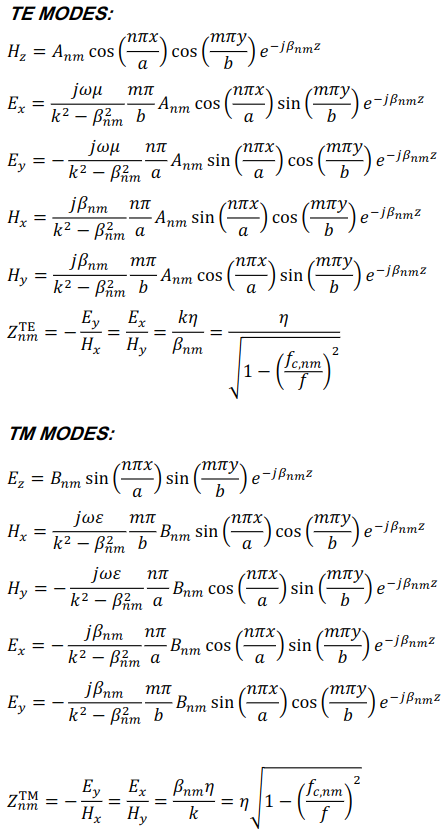
\includegraphics[width=\columnwidth]{tem_modes.png}

\end{multicols}
\end{document}